% Figure: delay catalogues in the log-delay coordinate. Referenced from
% rem:delay-dictionary (§3); the shape conditions it draws are proved in §7.
%
% Pedagogic point, one per panel: (a) in θ = log t the Lévy measure k(t)/t dt becomes
% one profile k~(θ) = k(e^θ) per unit log-delay; dilation is translation; the named
% families are SHAPES of the profile, and "nonincreasing" is the only constraint full
% covariance imposes. (b) the Dickman superposition: any nonincreasing profile is a
% unique positive stack of unit steps, one step = one Ein ray; the mixing measure
% ρ = -dk weighs the step released at each cutoff. Pure TikZ, no external file.
%
% The curve constants are chosen for legible composition, not computed from the
% families; the staircase in (b) is hand-placed under the sigmoid.

\begin{figure}[t]
\centering
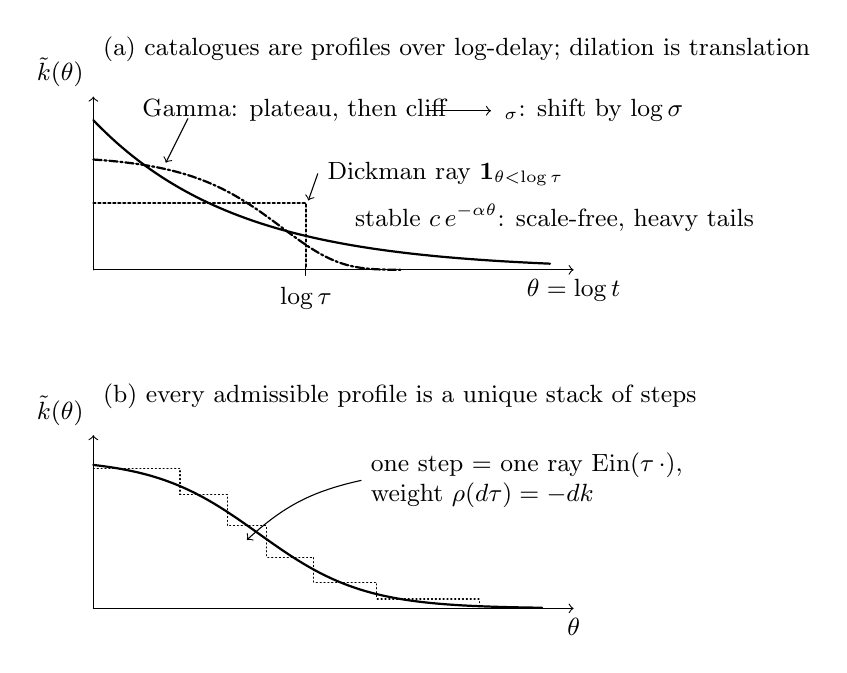
\begin{tikzpicture}[every node/.style={font=\small}, line cap=round]

% ---------- panel (a): the catalogue as a profile in log-delay ----------
\begin{scope}
  \node[anchor=west] at (-0.5,2.8) {(a) catalogues are profiles over log-delay; dilation is translation};
  % axes
  \draw[->] (-0.5,0) -- (5.6,0) node[anchor=north] {$\theta = \log t$};
  \draw[->] (-0.5,0) -- (-0.5,2.2) node[anchor=south east] {$\tilde k(\theta)$};
  % stable: exactly scale-free, exp(-alpha*theta) -- never cuts off (heavy tails)
  \draw[thick] plot[domain=-0.5:5.3, samples=80] (\x, {1.9*exp(-0.55*(\x+0.5))});
  \node[anchor=west] at (2.7,0.66) {stable $c\,e^{-\alpha\theta}$: scale-free, heavy tails};
  % Gamma: k(t) = e^{-t} -- plateau then cliff (finite moments)
  \draw[thick, densely dashdotted] plot[domain=-0.5:3.4, samples=80]
    (\x, {1.45*exp(-exp(1.4*(\x-1.9)))});
  \node[anchor=west] (gammalbl) at (0.0,2.02) {Gamma: plateau, then cliff};
  \draw[->] (0.7,1.92) -- (0.42,1.36);
  % Dickman ray: unit step to cutoff log tau
  \draw[thick, densely dotted] (-0.5,0.85) -- (2.2,0.85) -- (2.2,0.02);
  \node[anchor=west] (dicklbl) at (2.35,1.22) {Dickman ray $\mathbf{1}_{\theta < \log\tau}$};
  \draw[->] (dicklbl.west) -- (2.23,0.88);
  \draw (2.2,0.07) -- (2.2,-0.07); \node[anchor=north] at (2.2,-0.1) {$\log\tau$};
  % dilation = translation: arrow and caption side by side on the Gamma label's line,
  % keeping the band under the panel title empty (title and caption collided as
  % stacked lines -- 2026-09-01)
  \draw[->] (3.75,2.02) -- (4.55,2.02);
  \node[anchor=west] at (4.6,2.02) {$\dil_\sigma$: shift by $\log\sigma$};
\end{scope}

% ---------- panel (b): the Dickman superposition ----------
\begin{scope}[yshift=-4.3cm]
  \node[anchor=west] at (-0.5,2.7) {(b) every admissible profile is a unique stack of steps};
  \draw[->] (-0.5,0) -- (5.6,0) node[anchor=north] {$\theta$};
  \draw[->] (-0.5,0) -- (-0.5,2.2) node[anchor=south east] {$\tilde k(\theta)$};
  % a generic nonincreasing profile
  \draw[thick] plot[domain=-0.5:5.2, samples=80] (\x, {1.9/(1+exp(1.5*(\x-1.6)))});
  % inscribed staircase: steps released at successive cutoffs
  \draw[densely dotted]
    (-0.5,1.78) -| (0.6,1.45) -| (1.2,1.05) -| (1.7,0.65) -| (2.3,0.33) -| (3.1,0.12) -| (4.4,0);
  % annotation: one step = one Ein ray, weight rho(d tau)
  \node[anchor=south west, align=left] (steps) at (2.9,1.15)
    {one step $=$ one ray $\mathrm{Ein}(\tau\,\cdot)$,\\ weight $\rho(d\tau) = -dk$};
  \draw[->] (steps.west) to[bend right=15] (1.45,0.87);
\end{scope}

\end{tikzpicture}
\caption{Delay catalogues in the log-delay coordinate $\theta = \log t$, where the
Lévy measure $k(t)\,t^{-1}dt$ becomes the profile $\tilde k(\theta) = k(e^\theta)$
and dilation acts by translation. (a)~Full scale covariance requires only that the
profile be nonincreasing --- zooming out may only add delay intensity
(Lemma~\ref{lem:selfdecomposable-exponents}); within that freedom the named families
are shapes: the stable family is the exactly scale-free exponential profile, whose
slow decay is the heavy tail (Corollary~\ref{cor:semigroup-case}); the Gamma family
cuts long delays off at a cliff, buying finite moments; and the Dickman ray is a
log-uniform band of delays with a hard cutoff. (b)~The Dickman superposition
(Lemma~\ref{lem:dickman-superposition}): every nonincreasing profile is a unique
positive stack of unit steps, so every admissible family is a unique superposition of
drift and dilated Dickman subordinators, with mixing measure $\rho = -dk$
(Proposition~\ref{prop:extreme-rays}).}
\label{fig:delay-catalogue}
\end{figure}
